\section{}

\textbf{Tiempo de lectura:} \{s18-reading-time\}

\section{Dispositivos de
almacenamiento}\label{_dispositivos_de_almacenamiento}

Los ordenadores pueden almacenar información en diferentes soportes de
almacenamiento ---por ejemplo, en discos magnéticos, DVD o memorias de
estado sólido---. Cada uno tiene propiedades físicas diferentes que
pasamos a comentar brevemente a continuación.

\subsection{Discos magnéticos}\label{_discos_magnuxe9ticos}

Los discos magnéticos son el tipo principal de almacenamiento
secundario, generalmente en la forma de lo que se denominan discos
duros.

\begin{figure}
\centering
\includegraphics[keepaspectratio]{media/C18_almacenamiento/disco_duro_físico.jpg}
\caption{Disco duro --- Fuente:
\href{https://commons.wikimedia.org/wiki/File:Hard_Drive_(11644168395).jpg}{Wikipedia}}\label{fig-disco-duro-fuxedsico}
\end{figure}

Tal y como se puede apreciar en la
\hyperref[fig-disco-duro-fuxedsico]{Disco duro --- Fuente: } cada unidad
está compuesta por una serie de platos de forma circular recubiertos de
material magnético. La información se almacena grabándola magnéticamente
sobre los platos, para lo cual se utilizan unas cabezas de lectura que
«flotan» tanto por encima como por debajo de cada plato.

\begin{figure}
\centering
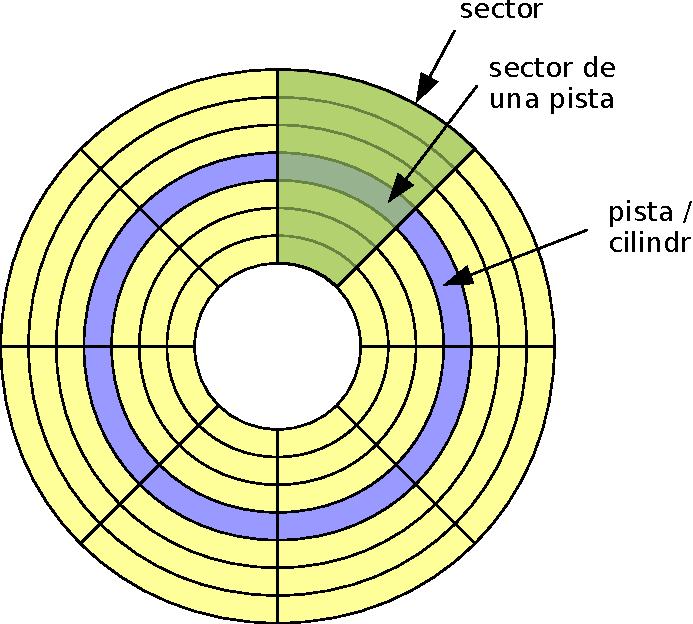
\includegraphics[width=0.8\textwidth]{media/C18_almacenamiento/disco_duro_lógico.pdf}
\caption{Estructura lógica de un disco
magnético.}\label{fig-disco-duro-luxf3gico}
\end{figure}

Desde el punto de vista lógico (véase la
\hyperref[fig-disco-duro-luxf3gico]{Estructura lógica de un disco
magnético.}) la superficie de cada plato está dividida en
\textbf{pista}{} circulares, cada una de las cuales se subdivide en
\textbf{sectores}{}. El conjunto de pistas formado por todas aquellas
que están situadas en la misma posición en los distintos platos se
denomina \textbf{{}cilindro}.

En estos dispositivos consume mucho más tiempo mover la cabeza de
lectura hasta el sector de interés, que la lectura y transferencia de
los datos almacenados a la memoria RAM. Por lo tanto, el tiempo de
acceso aleatorio al disco es mucho mayor que el de acceso secuencial.

\subsection{Discos ópticos}\label{_discos_uxf3pticos}

Los discos ópticos ---CD, DVD, BluRay, o cualquier otro medio similar---
consisten en un disco circular en el cual la información se almacena
haciendo uso de surcos microscópicos, que se leen haciendo incidir un
láser sobre una de las caras planas que lo componen.

En este tipo de discos la información se almacena siguiendo un recorrido
continuo en espiral que cubre la superficie entera del disco,
extendiéndose desde el interior hacia el exterior. Dado que el láser
siempre debe desplazarse sobre la espiral, el acceso aleatorio a los
datos es más lento que con otras tecnologías de disco.

\subsection{Memorias de estado
sólido}\label{_memorias_de_estado_suxf3lido}

Una memoria de estado sólido ---memoria USB o un SSD--- es un
dispositivo de almacenamiento que usa una memoria no volátil ---como las
\href{https://es.wikipedia.org/wiki/Memoria_flash}{memorias
\emph{flash}}--- para almacenar datos, en lugar de utilizar discos
ópticos o magnéticos.

En este tipo de memorias la información se almacena como en un vector
lineal de bytes, que se puede indexar aleatoriamente con la misma
eficiencia con la que se accede secuencialmente ---como ocurre con la
memoria RAM---. Sin embargo algunos dispositivos, de cara al resto del
sistema informático, emulan una interfaz y un modo de direccionamiento
similar al utilizado por los discos magnéticos ---es decir, usando
pistas, sectores y cilindros--- por temas de compatibilidad.

\section{Archivos y sistemas de
archivos}\label{_archivos_y_sistemas_de_archivos}

Teniendo en cuenta la gran diversidad de dispositivos de almacenamiento
que existen, para que el sistema informático sea cómodo de utilizar, el
sistema operativo proporciona una visión lógica uniforme de todos los
sistemas de almacenamiento. Es decir, abstrae las propiedades físicas de
los dispositivos de almacenamiento para definir una unidad de
almacenamiento lógico que sea útil para los usuarios. Esta unidad es el
\textbf{archivo}.

Un \textbf{{}archivo} o \textbf{{}fichero} es una colección de datos
relacionados, identificados por un nombre, que es tratada por el sistema
operativo como la unidad de información en el almacenamiento secundario.
Desde la perspectiva de los usuarios, un archivo es la unidad más
pequeña de almacenamiento. Es decir, los usuarios no pueden escribir
datos en el almacenamiento secundario a menos que estos se encuentren
dentro de un archivo.

El sistema operativo puede ofrecer esta abstracción gracias al
\textbf{sistema de archivos}{}. Este proporciona los mecanismos para el
almacenamiento de los datos y programas en archivos, tanto del propio
sistema operativo como los de todos los usuarios del sistema
informático.

Los sistemas de archivos están compuestos de dos partes claramente
diferenciadas:

\begin{itemize}
\item
  \textbf{Una colección de archivos}, cada una de las cuales almacena
  una serie de datos relacionados.
\item
  \textbf{Una colección de estructuras de metadatos}, que contienen
  información relativa a los archivos almacenados ---nombre, ubicación
  en el disco, permisos, entre otros--- y que se encarga de
  organizarlos; generalmente haciendo uso de una estructura de
  directorios.
\end{itemize}

\section{Volúmenes de datos}\label{_voluxfamenes_de_datos}

Los dispositivos de almacenamiento comentados anteriormente pueden ser
utilizados al 100\% con un único sistema de archivos. Sin embargo, en
ocasiones es interesante hacer divisiones con el objeto de disponer de
múltiples sistemas de archivos en el mismo dispositivo. Cada una de esas
divisiones es un \textbf{volumen}.

En otros casos interesa combinar divisiones o dispositivos de
almacenamiento completos para crear espacios de mayor tamaño ---también
denominados \textbf{volúmenes}--- cada una de las cuales puede albergar
un único sistema de archivos. Así que en general, utilizaremos el
término \textbf{{}volumen} para referirnos a un espacio de
almacenamiento que alberga un sistema de archivos, tanto si ese espacio
es una pequeña parte del espacio completo del dispositivo, como si se
trata de una estructura de mayor tamaño compuesta a partir de varios
dispositivos.

A continuación comentaremos brevemente las tecnologías utilizadas con
mayor frecuencia para construir estos volúmenes.

\subsection{RAID}\label{_raid}

La tecnología \textbf{{}RAID} (\emph{Redundant Array of Inexpensive
Disks}) permite combinar varios discos duros para mejorar las
prestaciones a través del paralelismo en el acceso o para mejorar la
fiabilidad a través del almacenamiento de información redundante. En
concreto se definen diversos \textbf{niveles RAID}, de entre los cuales
los más comunes son:

\begin{itemize}
\item
  En un \textbf{conjunto RAID 0} se distribuyen los datos
  equitativamente en bloques de tamaño fijo entrelazados entre dos o más
  discos, sin incluir ningún tipo de información redundante. Esto
  permite leer y escribir más datos al mismo tiempo, ya que se pueden
  enviar en paralelo peticiones a los distintos discos. Sin embargo, la
  fiabilidad es inversamente proporcional al número de discos, ya que
  para que el conjunto falle basta con que lo haga cualquiera de ellos.
\item
  En un \textbf{conjunto RAID 1} se crea una copia exacta ---en
  espejo--- de los datos en dos o más discos. El resultado es que,
  incluso con dos discos, se incrementa exponencialmente la fiabilidad
  respecto a tener uno solo, ya que para que el conjunto falle es
  necesario que lo hagan todos los discos. Adicionalmente, el
  rendimiento en las operaciones de lectura se incrementa linealmente
  con el número de copias, ya que los datos están disponibles en todos
  los discos al mismo tiempo, por lo que se pueden balancear las
  operaciones de lectura entre todos ellos.
\item
  En un \textbf{conjunto RAID 5} se distribuyen los datos
  equitativamente en bloques de tamaño fijo entrelazados entre dos o más
  discos y se utiliza uno adicional para almacenar la información de
  paridad de los bloques de una misma división. En RAID se denomina
  división o \emph{stripe} a la serie de bloques consecutivos, escogidos
  de cada uno de los discos del conjunto.

  El disco utilizado para almacenar el bloque de paridad cambia de forma
  escalonada de una división a la siguiente, de ahí que se diga que el
  bloque de paridad está distribuido. Algunos aspectos adicionales a
  tener en cuenta son que:

  \begin{itemize}
  \item
    Cada vez que se escribe un bloque de datos se debe actualizar el
    bloque de paridad. Por lo tanto las escrituras en un conjunto RAID 5
    son costosas en términos de operaciones de disco y tráfico.
  \item
    Los bloques de paridad no se leen durante las lecturas de datos, ya
    que eso reduciría el rendimiento. Solo se hace en caso de que la
    lectura de un sector falle, puesto que el sector en la misma
    posición relativa dentro de cada uno de los otros bloques de datos
    de la división y en el bloque de paridad se pueden utilizar para
    reconstruir el sector erróneo.
  \item
    En un conjunto RAID 5 el fallo de 2 discos provoca la pérdida
    completa de los datos. Esto significa que aunque se pueden añadir
    discos de manera ilimitada, eso no suele ocurrir, puesto que a más
    discos en el conjunto más probabilidad de que fallen dos de ellos.
  \end{itemize}
\item
  En un \textbf{conjunto RAID 6} se utiliza la misma estrategia que en
  RAID 5, pero en cada división hay dos bloques de paridad ---en lugar
  de uno--- en dos discos diferentes. Esto permite que fallen hasta dos
  discos sin perder los datos.
\item
  En un conjunto con niveles anidados se combinan varios niveles RAID
  básicos como si fueran capas superpuestas. Ejemplos típicos son:

  \begin{itemize}
  \item
    \textbf{RAID 0+1}, donde se hace un espejo de un conjunto RAID 0.
  \item
    \textbf{RAID 1+0} o \textbf{RAID 10}, donde diversos conjuntos en
    espejo se combinan en un RAID 0, aumentando la capacidad total.
  \item
    \textbf{RAID 50}, donde diversos conjuntos RAID 5 se combinan en un
    RAID 0, aumentando también la capacidad total.
  \end{itemize}
\end{itemize}

La implementación de RAID es otra de las áreas donde existen diversas
variantes:

\begin{itemize}
\item
  RAID puede implementarse en el hardware de la controladora de disco,
  de tal forma que solo los discos conectados a esta pueden formar parte
  de un conjunto RAID determinado. Esta solución es muy eficiente,
  especialmente cuando se utilizan niveles que requieren cálculo de la
  paridad, ya que se evita utilizar tiempo de CPU para ese trabajo. Sin
  embargo, estas controladoras son notablemente más caras que las que
  carecen de soporte para RAID.
\item
  RAID puede implementarse dentro del sistema operativo en lo que se
  denomina el \textbf{software de gestión de volúmenes}{}. En este caso
  las soluciones RAID con paridad son bastante lentas, por lo que
  normalmente solo se soportan los niveles RAID 0, 1, 10 o 0+1. Algunas
  controladoras de disco modernas que dicen venir con soporte RAID
  realmente implementan esta tecnología en software, a nivel del
  controlador de dispositivo, mientras que en el hardware solo se
  implementan unas características de apoyo mínimas. En algunos entornos
  se denomina a este tipo de implementaciones \emph{fakeRAID} o
  \emph{hostRAID}.
\end{itemize}

Cada conjunto RAID se comporta como una unidad de almacenamiento
independiente desde el punto de vista del resto del sistema, por lo que
se puede utilizar entero para albergar un único sistema de archivos. Sin
embargo, lo más común es dividirlo en regiones con el objeto de utilizar
múltiples sistemas de archivos o combinarlo en estructuras de mayor
tamaño, para lo cual se pueden utilizar alguna de las técnicas que
veremos a continuación.

\subsection{Particiones}\label{_particiones}

Un disco, un conjunto RAID o cualquier otro dispositivo de
almacenamiento se puede dividir en regiones para utilizar en cada una de
ellas un sistema de archivos diferente. A esas regiones se las conoce
comúnmente como \textbf{{}particiones}, \textbf{{}franjas} o
\textbf{{}minidiscos}.

Según la plataforma, existen diversas maneras de implementar el soporte
de particiones. Entre los sistemas de escritorio las tecnologías más
difundidas y utilizadas son la \textbf{MBR} (\emph{Master Boot Record})
y la \textbf{GPT} (\emph{GUID Partition Table}). En ambas se almacena,
en los primeros sectores del dispositivo de almacenamiento, una tabla
con una entrada por partición donde se guardan las direcciones del
primer y último sector de cada una de ellas en el dispositivo, así como
otra información. Eso es todo lo que necesita el sistema operativo para
determinar los límites de la región ocupada por cada sistema de
archivos.

\subsection{Volúmenes dinámicos}\label{_voluxfamenes_dinuxe1micos}

Según la tecnología que se utilice para particionar es posible
encontrarse con una serie de restricciones comunes:

\begin{itemize}
\item
  Limitado número de particiones que puede contener un mismo
  dispositivo.
\item
  Limitaciones o imposibilidad de redimensionar las particiones.
  Especialmente si el sistema operativo está en ejecución.
\item
  La imposibilidad de crear particiones que hagan uso de regiones libres
  en diferentes dispositivos de almacenamiento.
\end{itemize}

Para resolverlo, algunos sistemas operativos incluyen un
\textbf{software de gestión de volúmenes}{} que hace uso de tecnología
propia para superar estas limitaciones. Estas herramientas generalmente
permiten agrupar dispositivos completos, conjuntos RAID, particiones,
etc. y sobre ellos construir los volúmenes que sean necesarios. Estos
volúmenes pueden ser redimensionados ---en ocasiones sin tener que
detener la ejecución del sistema operativo--- y en caso de que haga
falta se pueden incluir dinámicamente nuevos dispositivos para
incrementar el espacio disponible. Además, como ya hemos comentado, el
software de gestión de volúmenes puede incluir alguna funcionalidad
propia de conjuntos RAID, con el objeto de mejorar las prestaciones, a
través del paralelismo en el acceso, o mejorar la fiabilidad, a través
del almacenamiento de información redundante.
